\documentclass[10pt]{beamer}
\usetheme{CambridgeUS}
\usepackage[utf8]{inputenc}
\usepackage[francais]{babel}
\usepackage[T1]{fontenc}
\usepackage{amsmath}
\usepackage{amsfonts}
\usepackage{amssymb}
\usepackage{graphicx}
\author{Dr Mory Ouattara\\  Data Science }
\title{Analyse Multivariée des Données}
\setbeamercovered{transparent} 
%\setbeamertemplate{navigation symbols}{} 
%\logo{} 
\institute{INPHB} 
\date{ } 
\subject{Analyse Multivariée} 
\begin{document}

\begin{frame}
\titlepage
\end{frame}

\begin{frame}
\tableofcontents
\end{frame}

\section{Données Multivariées}

\subsection{ }


%%%%%%%%%%%%%%%%%%%%%%%%%%%%%%%%%%
%%%%%%%%%%%%%%%%%%%%%%%%%%%%%%%%%%

%\section{Données Multivariées}

%\subsection{ }

\begin{frame}{Données Multivariées}

  
\centering 
 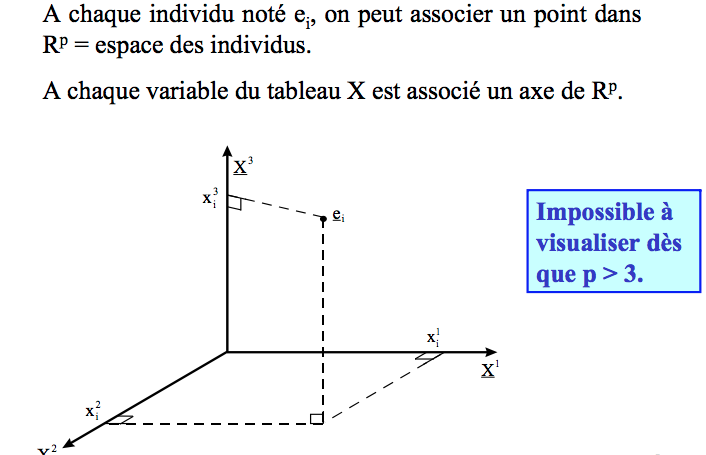
\includegraphics[scale=0.45]{Proj1.png} 
 

\end{frame}
%%%%%%%%%%%%%%%%%%%%%%%%%%%%%%%%%%
%%%%%%%%%%%%%%%%%%%%%%%%%%%%%%%%%%







\begin{frame}{Données Multivariées}

 Soit $x \in \mathbb{R}^p$ un vecteur aléatoire :
 
 $$ x=(\xi_1,\xi_2, \ldots, \xi_p )^T$$ où $v^T$ désigne la transposée du vecteur $v$  avec $\xi_j$ est une variable aléatoire\\~\\
 Un \textcolor{blue}{échantillon multidimensionnel} est une suite $x_1, \ldots, x_n$ de  réalisations aléatoires du vecteur $x$.\\~\\
 
 $x_{ij}$ désignera la j ème composante du vecteur $x_i$
 
\centering 
 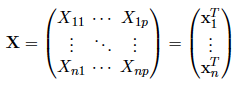
\includegraphics[scale=0.6]{X.png} 
 

\end{frame}
 
%%%%%%%%%%%%%%%%%%%%%%%%%%%%%%%%%

%\section{Statistiques}
\begin{frame}{Statistiques}

  \begin{enumerate}
  \item Les moyennes empiriques
  $$\bar{x_k}=\frac{1}{n}\sum_{i=1}^nx_{ki} \ k=1, \ldots, p $$ qui forment le vecteur 
  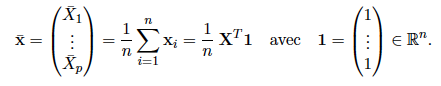
\includegraphics[scale=0.6]{X_bar.png} 
  \item
  Les covariances empiriques
  $$ s_{jk}=\frac{1}{n}\sum_{i}^n x_{ij}x_{ik}-\bar{x_j}\bar{x_k}  \  k,j=1, \ldots p $$ qui forment la matrice covariance empirique $ S=(S_{kj}) $
  \end{enumerate}
\end{frame}

 
 \begin{frame}{Statistiques}

  \begin{enumerate}
  \item[3] Les corrélations empiriques
  
  $$ r_{jk}=\frac{s_{jk}}{\sqrt{s_{jj}s_{kk}}}   \  k,j=1, \ldots p $$  qui forment la matrice de corrélation empirique
  $$ R=(r_{jk})_{k, j=1, \ldots p} $$ 
  \end{enumerate}
\end{frame}

\begin{frame}{Statistiques}
Il est facile de voir que  

$$ S=\frac{1}{n}\sum_{i=1}^nx_ix_i^T-\bar{x}\bar{x}^T=\frac{1}{n}XX^T-\frac{1}{n^2}X\textbf{1 1}^TX^T=\frac{1}{n}X^THX$$  

où $$ H=I_n-\frac{1}{n}\textbf{1 1}^T $$ est la matrice de centrage

\begin{enumerate}
\item \textit{Montrer que $H$ est un projecteur, i. e. $H = H^2$ et $H^T = H$. Sur quel sous-espace vectoriel de $\mathbb{R}^n$ projette-t-il ?}

\item \textit{Montrer la matrice de covariance empirique S est positive, en effet pour tout vecteur $R^p$.}

\end{enumerate}


\end{frame}



%%%%%%%%%%%%%%%%%%%%%%%%%%%%%%%%%
%%%%%%%%%%%%%%%%%%%%%%%%%%%%%%%%%

\section{Analyse en composantes principales (ACP)}
\begin{frame}{l’Analyse en Composantes Principales (ACP)}

L’Analyse en composantes principales (ACP) est une méthode de traitement des données multidimensionnelles qui poursuit les deux objectifs suivants :

\begin{enumerate}
\item \textcolor{blue}{Visualiser les données} (\textbf{Notion de distances entre individus})\\~\\
\item \textcolor{blue}{Réduire la dimension} effective des données \textbf{(en fonction de leurs corrélations)}.\\~\\
\end{enumerate}



\end{frame}



%%%%%%%%%%%%%%%%%%%%%%%%%%%%%%%%%
%%%%%%%%%%%%%%%%%%%%%%%%%%%%%%%%%
\begin{frame}{L’idée de l’Analyse en composantes principales (ACP)}


si $a = (a_1, \ldots ,a_p)^T \in R^p$ est une direction de projection.\\~\\

\begin{itemize}

\item Les données projetées $(a^T x_1, . . . ,a^T x_n)$ forment un échantillon de dimension 1.\\~\\

\item que l’on peut visualiser et qui est donc plus facile à interpréter que l’échantillon de départ $(x_1, \dots , x_n)$.\\~\\

\end{itemize}


\end{frame}

%%%%%%%%%%%%%%%%%%%%%%%%%%%%%%%%%
%%%%%%%%%%%%%%%%%%%%%%%%%%%%%%%%%
\begin{frame}{L’idée de l’Analyse en composantes principales (ACP)}

\centering

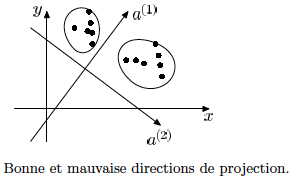
\includegraphics[scale=0.6]{ACP_ID.png} 

L’ACP a pour objectif de trouver un sous-espace linéaire de $\mathbb{R}^p$ de dimension $p* << p$ tel que la projection sur ce sous-espace “capte” presque toute la structure des données.


\end{frame}

%%%%%%%%%%%%%%%%%%%%%%%%%%%%%%%%%
%%%%%%%%%%%%%%%%%%%%%%%%%%%%%%%%%
\begin{frame}{L’idée de l’Analyse en composantes principales (ACP)}

L’Analyse en composantes principales (ACP) est une méthode de traitement des données multidimensionnelles qui poursuit les deux objectifs suivants :

 
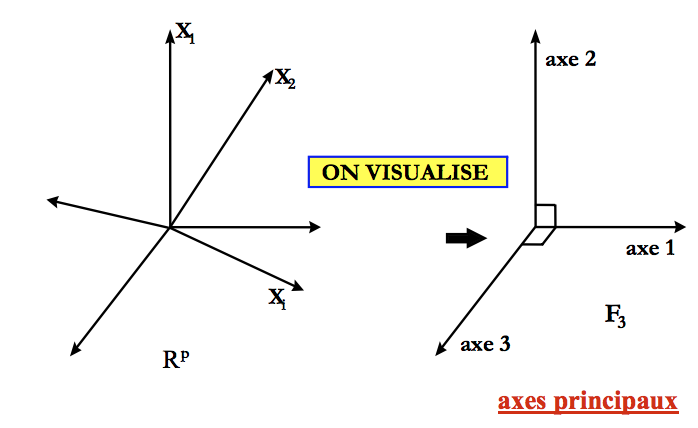
\includegraphics[scale=0.4]{Viz.png} 

\end{frame}


%%%%%%%%%%%%%%%%%%%%%%%%%%%%%%%%%
%%%%%%%%%%%%%%%%%%%%%%%%%%%%%%%%%
\begin{frame}{L’idée de l’Analyse en composantes principales (ACP)}

L’Analyse en composantes principales (ACP) est une méthode de traitement des données multidimensionnelles qui poursuit les deux objectifs suivants :

 
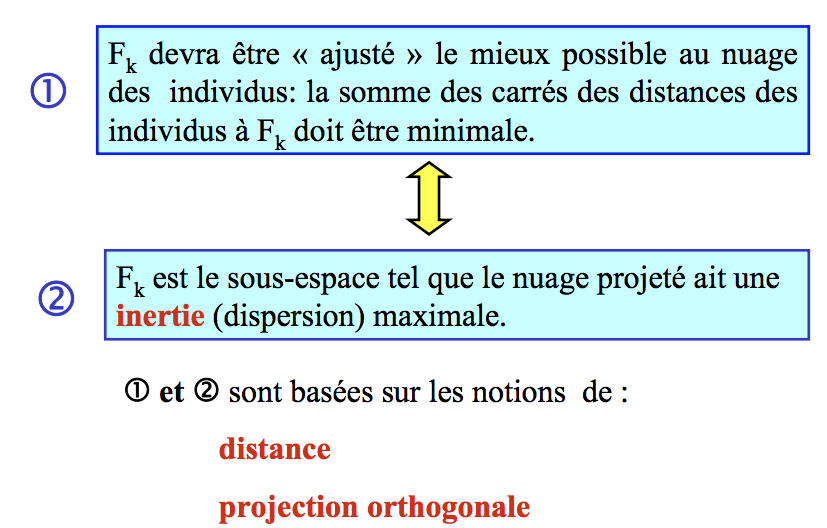
\includegraphics[scale=0.4]{Viz2.png} 

\end{frame}





%%%%%%%%%%%%%%%%%%%%%%%%%%%%%%%%%
%%%%%%%%%%%%%%%%%%%%%%%%%%%%%%%%%
\begin{frame}{ Critère de l'ACP}

L’idée de base de l’ACP est de chercher la direction  $\textbf{\textit{a}} \in \mathbb{R}^p$ qui maximise en \textit{\textbf{a}} la variance empirique de l’échantillon unidimensionnel $(a^T x_1, . . . ,a^T x_n)$


\centering
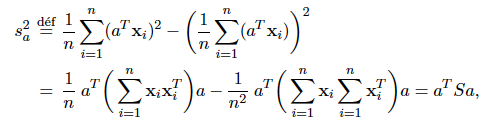
\includegraphics[scale=0.6]{Sa.png} 

la direction la plus intéressante $\hat{a}$ est une solution de 

$$\underset{a \in \mathbb{R}^p : \parallel a \parallel=1}{max}    a^TSa=\hat{a}^TS\hat{a} $$
ou 
$$ \hat{a}=\underset{a \in \mathbb{R}^p : \parallel a \parallel=1}{arg \ max} a^T Sa $$

\end{frame}

%%%%%%%%%%%%%%%%%%%%%%%%%%%%%%%%%
%%%%%%%%%%%%%%%%%%%%%%%%%%%%%%%%%

\begin{frame}{Décomposition spectrale}

Nous nous intéressons à la solution du problème suivant : 

$$ a^*=\underset{a \in \mathbb{R}^p : \parallel a \parallel=1}{arg \ max} Var (a^TX) \ avec \  E(\parallel X \parallel^2)<\infty$$

Soit $$ \Sigma =\Gamma \Lambda \Gamma^T $$ une décomposition spectrale de covariance 
 
\centering
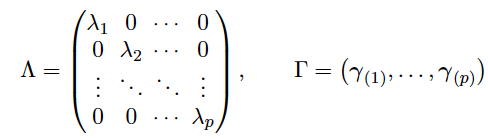
\includegraphics[scale=.4]{Decomp.png} 

Où les $\lambda_i$ sont les valeurs propres de $\Sigma$ rangées dans l'ordre croissant et  $$ \parallel \gamma_{(i)}  \parallel=1    \  avec \   \gamma_{(i)}^T \gamma_{(k)}=0 \  pour \  i \neq k $$ 

\end{frame}

%%%%%%%%%%%%%%%%%%%%%%%%%%%%%%%%%
%%%%%%%%%%%%%%%%%%%%%%%%%%%%%%%%%
\begin{frame}{Les Composantes principales $\eta_{(j)}$ }

\begin{block}{Composante principale $\eta_{(j)}$}
La variable aléatoire $\eta_{(j)} = \gamma_{(i)}^T(x-\mu) $ est dite j ème composante principale du vecteur aléatoire $x \in R^p$.
\end{block}


Les $\gamma_{(j)}$ sont les vecteurs propres de la matrice
de covariance $\Sigma$  du vecteur aléatoire $x$, on obtient : 


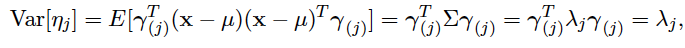
\includegraphics[scale=0.5]{VarEtaj.png}


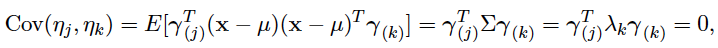
\includegraphics[scale=0.45]{CovEtaj.png}



\end{frame}

%%%%%%%%%%%%%%%%%%%%%%%%%%%%%%%%%

\begin{frame}{ ACP}

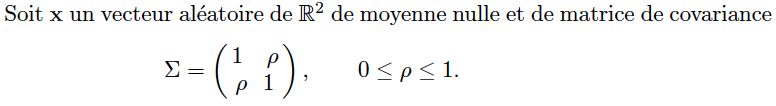
\includegraphics[scale=0.35]{ex1.png}

\end{frame}


%%%%%%%%%%%%%%%%%%%%%%%%%%%%%%%%%
\begin{frame}{Exemple ACP }

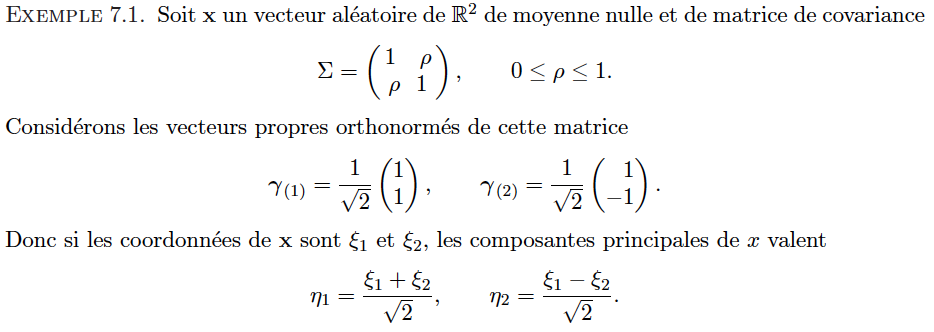
\includegraphics[scale=0.39]{ex.png}

\end{frame}



%%%%%%%%%%%%%%%%%%%%%%%%%%%%%%%%%
%%%%%%%%%%%%%%%%%%%%%%%%%%%%%%%%%
\begin{frame}{ Exemple ACP }

\begin{block}{Théorème}

Soit $x \in R^p$ un vecteur aléatoire tel que $E(\parallel  x \parallel) < \infty$. Alors  \textcolor{blue}{$\hat{a}= \gamma_{(1)}$} est
vérifie : 

 $$ Var(\hat{a}^TX)=\underset{a \in \mathbb{R}^p : \parallel a \parallel=1}{max} (a^TX)=\underset{a \in \mathbb{R}^p : \parallel a \parallel=1}{max} (a^T(X-\mu)) $$ 
 
\end{block}

\end{frame}



\begin{frame}{ACP }

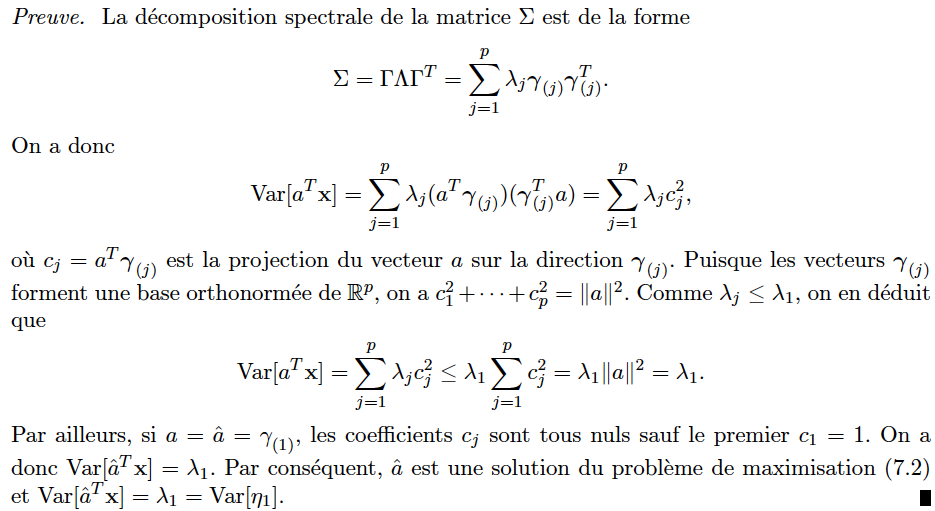
\includegraphics[scale=0.37]{Thee.png}

\end{frame}


%%%%%%%%%%%%%%%%%%%%%%%%%%%%%%%%%
%%%%%%%%%%%%%%%%%%%%%%%%%%%%%%%%%
\begin{frame}{Étude des corrélations }

 On définit la variance totale de $x$ par $$ E(\parallel  X-\mu\parallel^2)=E(X-\mu)^T(X-\mu)=E(X-\mu)^T\Gamma\Gamma^T (X-\mu)$$ avec 
 
 \centering 
 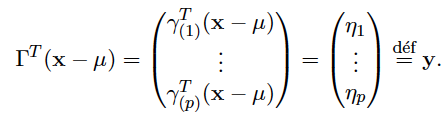
\includegraphics[scale=0.5]{Gamma.png}
 
 Compte tenu de ces notations et de l’égalité 
 $E(\eta_i^2) = \lambda_i$, on obtient 
 
$$ E(\parallel  X-\mu\parallel^2)=E(\eta_1^2+\ldots +\eta_p^2)$$ 

\end{frame}


%%%%%%%%%%%%%%%%%%%%%%%%%%%%%%%%%


%%%%%%%%%%%%%%%%%%%%%%%%%%%%%%%%%

\begin{frame}{ACP }


\begin{Large}
\textcolor{blue}{Donc: Comment détermine t-on le meilleur sous espace de projection ?}
\end{Large}

\end{frame}


%%%%%%%%%%%%%%%%%%%%%%%%%%%%%%%%%

%%%%%%%%%%%%%%%%%%%%%%%%%%%%%%%%%

%\section{Étude des corrélations}

\begin{frame}{Part de variance expliqué }

 \begin{block}{Part de variance expliqué}
 
 On appelle part de la variance totale de x expliquée par les k
premières composantes principales $(\eta_1, \ldots, \eta_k)$ la 

quantité  $$ \frac{\sum_{j=1}^K\lambda_j}{\sum_{j=1}^p\lambda_j} $$ 
 
 \end{block}

\end{frame}

%%%%%%%%%%%%%%%%%%%%%%%%%%%%%%%%%
%%%%%%%%%%%%%%%%%%%%%%%%%%%%%%%%%

\begin{frame}{ Choix du bon nombre d'axe}


 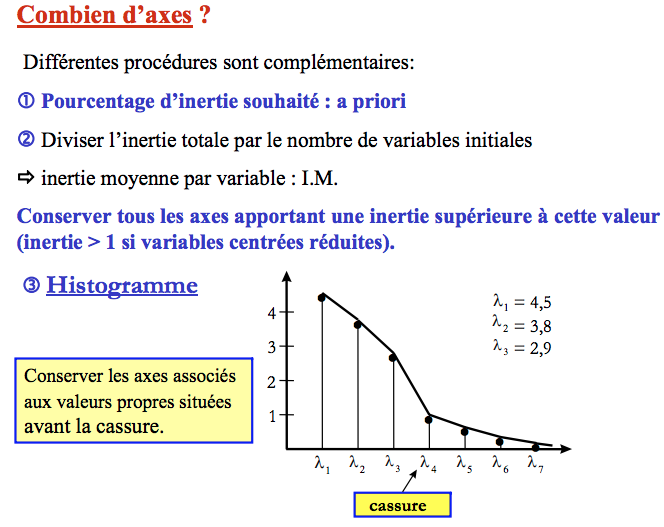
\includegraphics[scale=0.4]{Kaiser.png}

\end{frame}


%%%%%%%%%%%%%%%%%%%%%%%%%%%%%%%%%
%%%%%%%%%%%%%%%%%%%%%%%%%%%%%%%%%

\begin{frame}{Lien entre $\eta_j$ et $\xi_i$}

  
  Calculons d’abord la matrice de covariance des vecteurs aléatoires $x$ et $y$.
  
  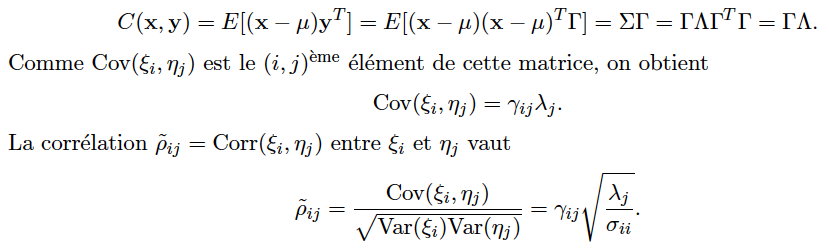
\includegraphics[scale=0.4]{EtaVar.png}
  
  
\end{frame}


%%%%%%%%%%%%%%%%%%%%%%%%%%%%%%%%%

%%%%%%%%%%%%%%%%%%%%%%%%%%%%%%%%%
\subsection{Lien entre $\eta_j$ et $\xi_i$}
\begin{frame}{Lien entre $\eta_j$ et $\xi_i$}

  \begin{block}{Proposition}
  
  Soit $x \in R^p$ un vecteur aléatoire, tel que $E(\parallel x \parallel^2) < \infty$ et $\sigma_{ii} > 0$ pour tout $i = 1, \ldots ,p$. 
 
  Alors, 
  
  $$\sum_{j=1}^p \tilde{\rho}^2_{ij} =1$$
  
  \end{block}
 
  On appelle $ \tilde{\rho}^2_{ij} $ part de variance de la variable $\xi_i$ expliquée par la $j$ ème composante principale $\eta$ .
  
  Pour tout sous-ensemble $J$ de $ {1, . . . ,p}$,
  $$\sum_{j \in J} \lambda_j=\sum_{j=1}^p \sigma_{ii}\tilde{\rho}^2_{iJ} \ avec \  \tilde{\rho}^2_{iJ} = \sum_{j \in J}{\rho}^2_{ij} $$
\end{frame}

%%%%%%%%%%%%%%%%%%%%%%%%%%%%%%%%%
%%%%%%%%%%%%%%%%%%%%%%%%%%%%%%%%%

\begin{frame}{Lien entre $\eta_j$ et $\xi_i$}


 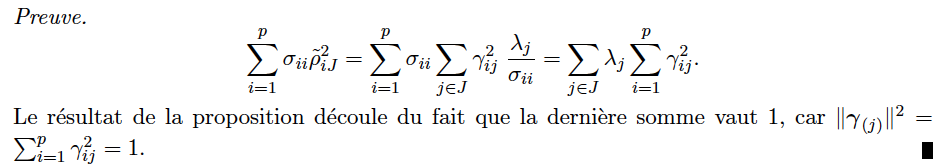
\includegraphics[scale=0.37]{Rho_ij.png}


\end{frame}

%%%%%%%%%%%%%%%%%%%%%%%%%%%%%%%%%
%%%%%%%%%%%%%%%%%%%%%%%%%%%%%%%%%
\subsection{Disque de corrélation}
\begin{frame}{Disque des corrélations}

  \begin{block}{Proposition}
  
  
  Soient $\xi_i$ et $\xi_k$ deux variables entièrement expliquées par les deux premières composantes principales, i.e.
  
  $$ \tilde{\rho_{i1}}^2 + \tilde{\rho_{i2}}^2=1 \ et  \  \tilde{\rho_{k1}}^2 + \tilde{\rho_{k2}}^2=1 $$
  
  Alors, la corrélation de $\xi_i$ et $\xi_k$ est donnée par la formule 
  
  $$  {\rho_{ik}}  = \tilde{\rho_{i1}}   \tilde{\rho_{k1}}  +  \tilde{\rho_{i2}}   \tilde{\rho_{k2}}  = cos(\varphi), $$

où $\varphi$ est l'angle formé par les vecteurs $(\tilde{\rho_{i1}}, \tilde{\rho_{i2}})$ et $(\tilde{\rho_{k1}}, \tilde{\rho_{k1}})$.
  
  \end{block}
 

\end{frame}
%%%%%%%%%%%%%%%%%%%%%%%%%%%%%%%%%
%%%%%%%%%%%%%%%%%%%%%%%%%%%%%%%%%

\begin{frame}{Disque des corrélations}

\centering 

 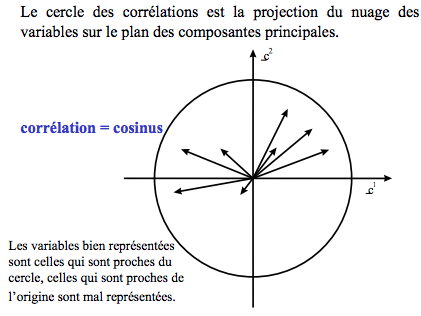
\includegraphics[scale=0.7]{Correlation.png}


\end{frame}


%%%%%%%%%%%%%%%%%%%%%%%%%%%%%%%%%
%%%%%%%%%%%%%%%%%%%%%%%%%%%%%%%%%
\subsection{Individus et variables supplémentaires }



\begin{frame}{ Variables }

 \begin{itemize}
 \item   On calcule le coefficient de corrélation entre la variable supplémentaire et les composantes principales. 
 
 \item Ceci permet sa représentation sur le cercle des corrélations.
 
 \end{itemize}


\end{frame}


%%%%%%%%%%%%%%%%%%%%%%%%%%%%%%%%%
%%%%%%%%%%%%%%%%%%%%%%%%%%%%%%%%%
 

\begin{frame}{ Individus }

 \begin{itemize}
 \item   Individu de poids nul ne participant pas à l’analyse  
 
\item Appliquer aux coordonnées de l’individu les expressions
définissant les composantes principales.
 \end{itemize}


\end{frame}

\subsection{Cas Pratique}
\begin{frame}{ Cas pratique : Campagne National Logement 2005}
\centering 
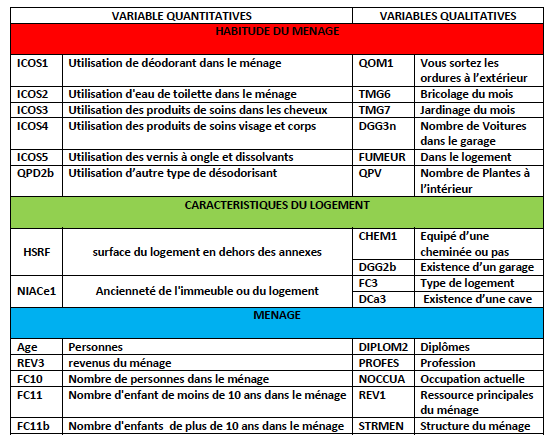
\includegraphics[scale=0.5]{CNL1} 

\end{frame}


\begin{frame}{ Cas pratique : Corrélation entre variables }
\centering 
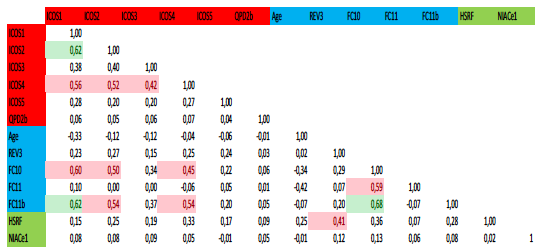
\includegraphics[scale=0.5]{CNL2} 

\end{frame}

\begin{frame}{ Cas pratique : Inertie des axes}
\centering 
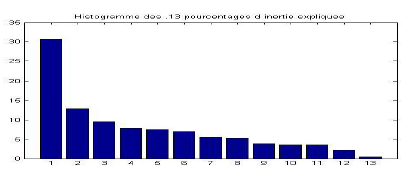
\includegraphics[scale=0.7]{CNL3} 

\end{frame}


\begin{frame}{ Cas pratique : Variables dans le 1er Plan  }
\centering 
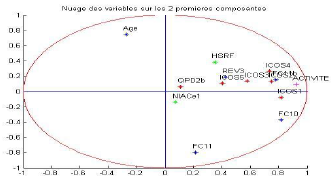
\includegraphics[scale=0.7]{CNL4} 

\end{frame}

\begin{frame}{ Cas pratique :  $\tilde{\rho}_{ij}$}
\centering 
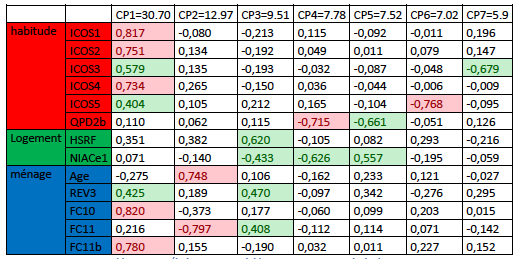
\includegraphics[scale=0.6]{CNL5} 

\end{frame}


\begin{frame}{ Cas pratique :  Contribution des individus}
\centering 
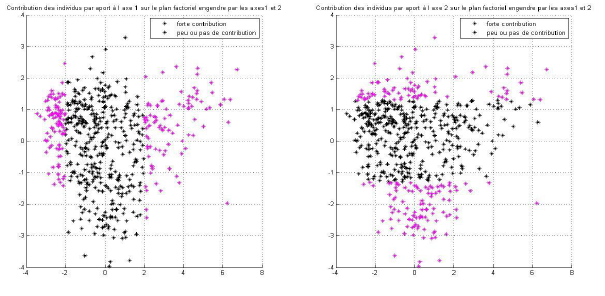
\includegraphics[scale=0.6]{CNL6} 

\end{frame}





\section{L'Analyse des Correspondances Simples (AFC)}
\begin{frame}
\centering
 \begin{Large}
 
 
L'Analyse des Correspondances Simples  \\



A F C
\end{Large}





\end{frame}



%%%%%%%%%%%%%%%%%%%%%%%%%%%%%%%%
\subsection{Test Khi2}
%\subsection{Problématique}
\begin{frame}{Structure de base des données}
Objective : mesurer des liaisons entre deux variables qualitatives :\textcolor{blue}{Khi-deux}\\
exemple : 
Il s’agit de tester l’indépendance de deux variables qualitatives.
Y a-t-il indépendance entre :


\begin{itemize}
\item la catégorie socioprofessionnelle et le vote à l'élection
présidentielle ?
\item  le niveau d’études et les journaux lus ?

\item Que pensez vous de cette affirmation : \textit{On en a assez de ceux qui bloquent la vie du pays par leurs revendications par les armes.}

\begin{enumerate}
\item  pas du tout d'accord
\item pas tellement d'accord 
\item bien d'accord 
\item entièrement d'accord
\end{enumerate}
\end{itemize}

 
\end{frame}

\begin{frame}{Structure de base des données}
\centering
Existe-t- il un lien entre les réponses et la tendance politique ?   
\begin{table}
\begin{tabular}{|c|c|c|c|c|c|c|}
\hline 
Tendance Politique & 1 & 2 & 3 & 4 & 5 & Total \\ 
\hline 
PIT & 714 & 71 & 0 & 143 & 71 & 1000 \\ 
\hline 
FPI & 284 & 216 & 199 & 174 & 127 & 1000 \\ 
\hline 
MFA & 87 & 106 & 228 & 335 & 244 & 1000 \\ 
\hline 
RDR & 16 & 86 & 156 & 271 & 471 & 1000 \\ 
\hline 
PDCI & 71 & 71 & 0 & 214 & 643 & 1000 \\ 
\hline 
Indifférent & 82 & 120 & 244 & 301 & 263 & 1000 \\ 
\hline 
Non Reponse & 88 & 124 & 269 & 285 & 233 & 1000 \\ 
\hline 
\end{tabular} 
\end{table}

 
\end{frame}

%\subsection{Le tableau de contingence noté  N}




\begin{frame}{Le tableau de contingence}
\begin{figure}
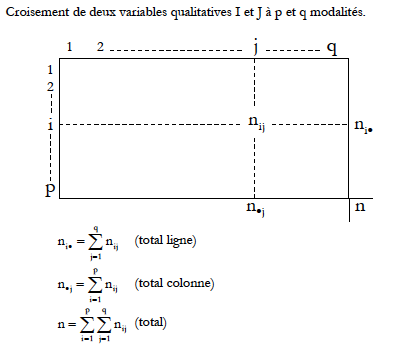
\includegraphics[scale=0.6]{Exemple3.png}  
\end{figure}
\end{frame}

 

 
\begin{frame}{Profils lignes - profils-colonnes - profils
marginaux}
\begin{figure}
\includegraphics[scale=0.7]{exemple9.png}  
\end{figure}
\end{frame}



%\begin{frame}{}
%
%\begin{figure}
%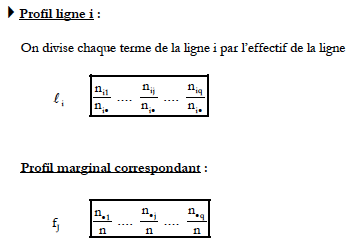
\includegraphics[scale=0.7]{Exemple4.png}  
%\end{figure}
%
%%\textcolor{blue}{Si les deux variables qualitatives I et J étaient indépendantes, les profils lignes seraient tous identiques, et donc identiques au profil marginal correspondant.}
%\end{frame}


\begin{frame}{Profils lignes - profils-colonnes - profils
marginaux}

\textcolor{blue}{Si les deux variables qualitatives I et J étaient indépendantes, les profils lignes seraient tous identiques, et donc identiques au profil marginal
correspondant.}\\~\\

$$Independance \Rightarrow \frac{n_{ij}}{n_{i \bullet}}=\frac{n_{\bullet j}}{n} \Rightarrow n_{ij}=\frac{n_{\bullet j}*n_{i \bullet}}{n}$$\\~\\

\end{frame}


\begin{frame}{Profils lignes - profils-colonnes - profils
marginaux}

\begin{itemize}
\item  On pouvait établir la relation précédente en raisonnant sur les profils colonnes.
 
\begin{figure}
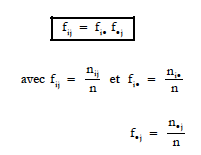
\includegraphics[scale=0.7]{Exemple5.png}  
\end{figure}
\end{itemize}

\textcolor{blue}{Elle exprime clairement que dans le cas de l’indépendance le tableau de contingence est entièrement déterminé par ses marges
}
\end{frame}

\begin{frame}{  Khi-deux}
\begin{itemize}
\item Pour chaque case, on peut donc calculer le nombre de cas attendus \textcolor{blue}{(sous hypothèse d’indépendance)}
$n_{ij}=\frac{n_{\bullet j}*n_{i \bullet}}{n} $\\~\\~\\

\item On peut comparer les nombres de cas attendus $E_{ij}$ aux nombres observés.

\begin{figure}
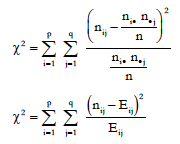
\includegraphics[scale=0.8]{Exemple6.png}  
\end{figure}
\end{itemize}
\end{frame}
%%%%%%%%%%%%%%%%%%%%


\begin{frame}{Test Khi-deux}

Si les deux variables sont réellement indépendantes, cette expression suit une distribution du Khi-deux avec un nombre de degrés de liberté égal
à : $(p -1) (q -1)$\\~\\

Dans une table on lit $\chi_{\alpha,k}^2$ valeur ayant une probabilité
$\alpha$ d’être dépassée pour une distribution du khi-deux avec $k = (p-1) (q -1)$ degrés de liberté.\\~\\~\\

\begin{enumerate}

\item Si $\chi^2\leq \chi_{\alpha,k}^2$  On accepte $H_o$ : independance \\~\\

\item  Si $\chi^2 > \chi_{\alpha,k}^2$  On rejette $H_o$ : independance \\~\\

\end{enumerate}

\end{frame}
%%%%%%%%%%%%%%%%%%%%%%%%%%%%%%%
\begin{frame}{Pratique sous logiciel statistique}

\begin{itemize}
\item  Calcul du $\chi^2$ associé au tableau de contingence noté $\chi^2_{obs}$.

\item Probabilité pour une v.a. suivant une loi du khi-deux à
$(p -1) (q -1)$ d.d.l. de dépasser $\chi^2_{obs}$.

\begin{figure}
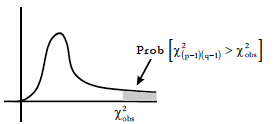
\includegraphics[scale=0.8]{exemple7.png}  
\end{figure}

\end{itemize}


\textcolor{blue}{Si cette probabilité est faible (en général < 5 \%), on rejette l’hypothèse d’indépendance entre les deux variables qualitatives.}


\end{frame}


\subsection{L'analyse des correspondances simples}
 
%%%%%%%%%%%%%%%%%%%%%%%%%%%%%%%
%\subsection{Notations et présentation}
%%%%%%%%%%%%%%%%%%%%%%%%%%%%%%%%%

\begin{frame}{Représentation des profils lignes}
\begin{itemize}
\item Les profils lignes sont considérés comme des individus.\\
\item Les p profils-lignes forment un nuage de p points dans $R^q$\\

\item A chaque profil-ligne est associé un poids égal à sa fréquence marginale profil ligne poids
$f_{i \bullet}$.
\end{itemize}
On note $N(I)$ le nuage de points formé des profils-lignes pondérés :
$( l_i; f_{i \bullet})$

Le centre de gravité g est défini par : $$ g_l=\sum_{i=1}^p f_{i \bullet}l_i$$

La jième coordonnée de $g_l$ vaut $f_{\bullet j}$\\~\\~\\

\textcolor{blue}{$g_l$ = profil marginal de la variable J (à q modalités) $g_l=f_J$}

\end{frame}
%%%%%%%%%%%%%%%%%%%%%%%%
\begin{frame}{Représentation des profils colonnes}
\begin{figure}
\includegraphics[scale=0.7]{exemple10.png}  
\end{figure}
\end{frame}
%%%%%%%%%%%%%%%%%%%%%%%%%%
\begin{frame}{}
\begin{figure}
\includegraphics[scale=0.5]{exemple11.png}  
\end{figure}
\end{frame}

%%%%%%%%%%%%%%%%%%%%%%%%%%%%
\begin{frame}{Métrique du $\chi 2$}

\begin{itemize}
\item Pour les profils lignes :\\

$$d^2_{\chi^2}(l_i,l_i')=\sum_{j=1}^{q}\frac{n}{n_{\bullet j}}(\frac{n_{ij}}{n_{i \bullet}}-\frac{n_{i'j}}{n_{i' \bullet}})^2  $$

\begin{itemize}
\item Donne un poids important aux différences portant sur les
petits pourcentages.
\item  Vérifie le principe d’équivalence distributionnelle : si deux
colonnes ont le même profil, on les réunit en une seule
d’effectif somme sans modifier les distances entre profils lignes.
\end{itemize}

\item Pour les profils-colonnes :

$$d^2_{\chi^2}(c_j,c_j')=\sum_{j=1}^{q}\frac{n}{n_{i \bullet }}(\frac{n_{ij}}{n_{\bullet j}}-\frac{n_{ij'}}{n_{ \bullet j'}})^2  $$       
       
\end{itemize}
\end{frame}
%%%%%%%%%%%%%%%%%%%%%%%%%%%%%
\begin{frame}{Inertie du nuage N(I)}
$I_{N(I)}$  l’inertie du nuage$ N(I)$ calculée par rapport
au centre de gravité $f_J$ vaut $$\frac{\chi^2}{n}$$

où $\chi^2=$ Khi-deux associé au tableau de contingence étudié.\\~\\~\\

\textcolor{blue}{On obtient le même résultat pour l’inertie du nuage N(J).} \\

Notons : 

\centering 

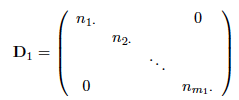
\includegraphics[scale=0.5]{D1.png} 
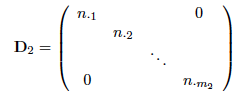
\includegraphics[scale=0.5]{D2.png} 

\end{frame}



\subsection{ACP du nuage des profils lignes-profils colonnes }
\begin{frame}{l’A.C.P. du nuage des profils-lignes :}
\begin{itemize}

\item Les données profils-lignes jouent le rôle d'individus 

$$ X= D_1^{-1}N$$

\item La métrique utilisée pour le calcul des distances entre
individus  $$ M=nD_2^{-1} \text{ et le poids } D= \frac{D_1}{n}$$

\item Les Facteurs principaux $u_k$ du nuage des profils-lignes N(I) sont vecteurs propres de $$MX'DX=(nD_2^{-1}) (D_1^{-1}N)'(\frac{D_1}{n})(D_1^{-1}N)=D_2^{-1}N'D_1^{-1}N$$ 

On a donc pour chaque axe principal $k$

 $$D_2^{-1}N'D_1^{-1}Nu_k=\lambda_ku_k$$

\item La composante principale $a_k$  associée au facteur $u_k$ est  vecteur propre de  :  $$D_1^{-1}N'D_2^{-1}N$$
\end{itemize}
\end{frame}

%\subsection{ACP du nuage des profils lignes-profils colonnes }
\begin{frame}{l’A.C.P. du nuage des profils-colonnes :}
Analyse des profils-colonnes on échange les indices 1 et 2
et on transpose N. \\

On notera $b_k$ les composantes principales. \\ 
\centering 
\textcolor{blue}{Comparaison Lignes-Colonnes}
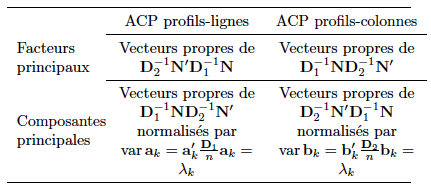
\includegraphics[scale=.7]{Synthese.png} 

\end{frame}


%%%%%%%%%%%%%%%%%%%%%%%%%

%\subsection{ Lien entre les deux analyses }



\begin{frame}{Abandon du principe barycentrique}

Les modalités de chaque ensemble sont représentées par les :

$$a^k_i,  i=1, \ldots, p$$

$$b^k_j ,  j=1, \ldots, q $$

Cette représentation permet de déterminer les proximités entre
certains éléments de I et certains éléments de J (\textcolor{blue}{compte tenu de la
qualité de la représentation}).

\end{frame}



\begin{frame}{Formules de transition}

En notant $b_j$ et $a_i$ les $j^{eme}$ et $i^{eme}$ coordonnées des composantes principales \textit{b} et \textit{a} associées à la même valeur propre $\lambda$ : 

$$ \sqrt{\lambda}b_j=\sum_{i=1}^p\frac{n_{ij}}{n_{\bullet j}}  a_i$$

$$ \sqrt{\lambda}a_i=\sum_{j=1}^q\frac{n_{ij}}{n_{i \bullet }}  b_j$$

\textcolor{blue}{À $\lambda$ près, la coordonnée d’une modalité i d’une variable est la moyenne des coordonnées des catégories de l’autre variable pondérées par les fréquences conditionnelles du profil de i.}
\end{frame}



%\subsection{Aides à l’interprétation : identiques à celles de l’A.C.P.}
\begin{frame}{Contributions}
\begin{figure}
\includegraphics[scale=0.6]{exemple16.png}  
\end{figure}
\end{frame}

\begin{frame}{Cosinus carrés}
\begin{figure}
\includegraphics[scale=0.6]{exemple17.png}  
\end{figure}

\end{frame}



\begin{frame}{Aspects pratiques de l’interprétation}

\begin{itemize}
\item L’interprétation peut se faire à partir des représentations graphiques (en s’assurant de la qualité de représentation de chaque modalité à
l’aide des cos2).\\~\\~\\
\item Quand le nombre de modalités est élevé, il est conseillé d’éditer d’abord le graphique des profils-lignes, puis celui des profilscolonnes, enfin la représentation simultanée.\\~\\~\\

\item Les profils ayant des poids différents la lecture de leurs
contributions à l’inertie de chaque axe s’avère très utile.\\~\\~\\

\item On peut repérer les profils dont la contribution est supérieure au poids
\end{itemize}
\end{frame}

\subsection{Cas pratique}

\begin{frame}{Exemples : Données CNL 2005}
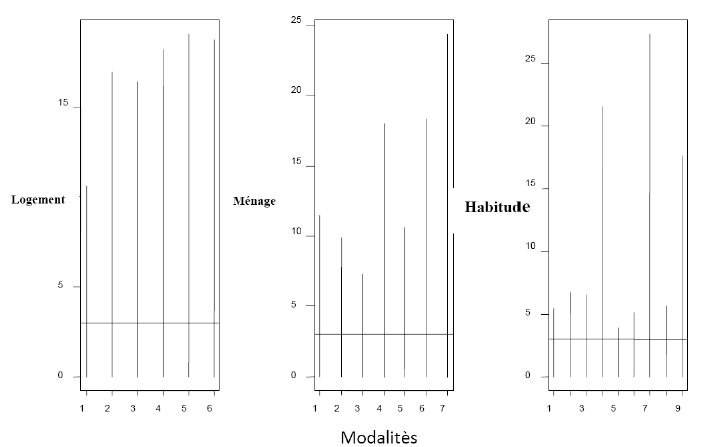
\includegraphics[scale=.5]{CNL8} 
Fréquences par modalité 
\end{frame}



\begin{frame}{Exemples : Test du Khi2}
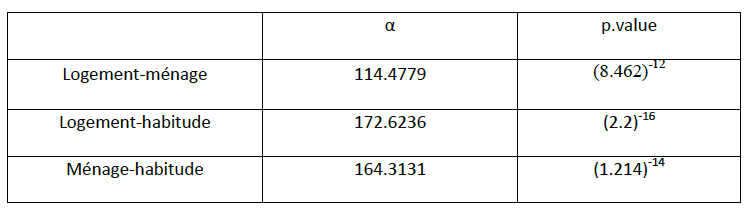
\includegraphics[scale=.45]{CNL9} 



S'en suit l'étude des liens entre les modalités.
\end{frame}
%%%%%%%%%%%%%%%%%%%%%%%%%%%%%%%%%%%%%%%%%%%%

\begin{frame}{Exemples : Logement Vs Ménage}
\centering 

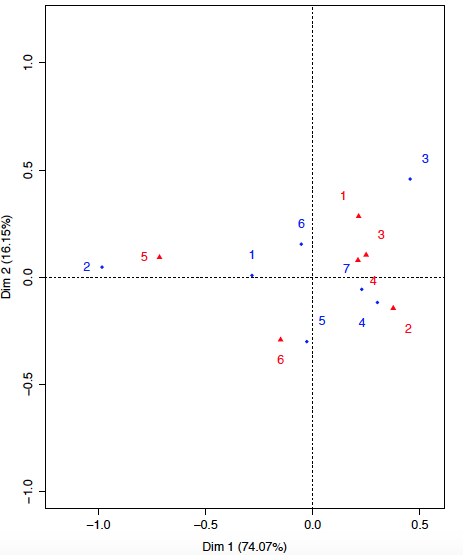
\includegraphics[scale=.4]{CNLAFC} 



S'en suit l'étude des liens entre les modalités.
\end{frame}

%%%%%%%%%%%%%%%%%%%%%%%%%%%%%%%%%%%%%%%%%%%%
%%%%%%%%%%%%%%%%%%%%%%%%%%%%%%%%%%%%%%%%%%%%

\section{Analyse des correspondances multiples (ACM)}


\begin{frame}{ Analyse des Correspondances Multiples }
\begin{itemize}
\item Étendre l'AFC au cas de $p \geq 2$ variables  $\xi_1, \xi_2,  \ldots, \xi_p$ à   $ m_1, \ldots, m_p $ modalités\\

\begin{table}
\begin{tabular}{ccccc}

 & $\xi_1$& $\ldots$ & $ \xi_p$& variables \\
 & $m_1$ & \ldots  &$m_p$ & modalités 
 
\end{tabular} 
\end{table}

 Utile pour l'exploration d'enquêtes où les questions sont à réponses multiples.\\~\\
\item L’analyse des correspondances utilise une table
de contingence qui est difficilement généralisable au cas
$p \geq 2$ .\\~\\
\end{itemize}

\textcolor{blue}{Trouver un moyen différent d'analyser $p > 2$
variables et vérifier que les résultats sont comparables à l’AFC pour p = 2.}
 

\end{frame}


%%%%%%%%%%%%%%%%%%%%%%%%%%%%%%%%%%%

\begin{frame}{ Données}
 
 \begin{itemize}
 \item \textbf{Données brutes} :  chaque individu est décrit par les numéros
des modalités qu’il possède pour chacune des p variables $\xi_j$..\\~\\

\textcolor{red}{Impossible de faire des calculs sur ce tableau :  valeurs arbitraires.}.\\~\\


\item Une forme mathématique utile pour les calculs est alors \textcolor{blue}{le tableau disjonctif des indicatrices des p variables} obtenu en juxtaposant les p tableaux d'indicatrices de chaque variable $\mathcal{X}_i$\\~\\

 \item  \textbf{Tableau disjonctif } : Remplacer la j-ième colonne par $m_j$ colonnes d'indicatrices : mettre  un zéro dans chaque colonne, sauf celle correspondant à la modalité de l’individu i qui
reçoit 1.
 \end{itemize}

 


\end{frame}


%%%%%%%%%%%%%%%%%%%%%%%%%%%%%%%%%%%
%%%%%%%%%%%%%%%%%%%%%%%%%%%%%%%%%%%





\subsection{Présentation Formelle}

\begin{frame}{Technique de description de données qualitatives}

n individus décrits par p variables qualitatives\\

\begin{table}
\begin{tabular}{ccccc}

 & $\mathcal{X}_1$& $\ldots$ & $ \mathcal{X}_p$& variables \\
 & $m_1$ & \ldots  &$m_p$ & modalités 
 
\end{tabular} 
\end{table}

\begin{itemize}
\item \textcolor{blue}{L'A.C.M. décrit les relations deux à deux entre p variables qualitatives à travers une représentation des groupes d'individus correspondant aux diverses modalités.} .\\~\\

\item Cette méthode est particulièrement bien adaptée à l'exploration d'enquêtes.
\end{itemize}

\end{frame}



\begin{frame}{Données  }

\textbf{Exemple} 

On interroge 6 personnes sur la couleur de leurs
cheveux (CB, CC et CR pour blond, châtain et roux), la couleur
de leurs yeux (YB, YV et YM pour bleu, vert et marron) et leur
sexe (H/F).   Les tableaux brut (ci-dessous à gauche) sont équivalents aux tableaux disjonctifs (à droite).\\~\\

\centering 
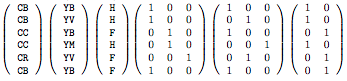
\includegraphics[scale=0.8]{disj.png} 


\end{frame}



\begin{frame}{Tableau disjonctif et tableau de contingence}

A chaque variable $\xi_j$  est associée un tableau disjonctif $X_j (n \times m_j)$. 

Pour 2 variables $\xi_j$  et $\xi_l$ le tableau de contingence  est donné par : 


\begin{table}
\begin{tabular}{cccccc}

 & $\mathcal{X}= {X}_j\vert  {X}_l$& $N_{j'l}={X}_j' {X}_l$&  ${X}_j' {X}_j$& ${X}_l' {X}_l$ \\
 &Disjonctifs&Contingence&Marge $\xi_j$&Marge $\xi_l$
 
\end{tabular} 
\end{table} 

\centering
 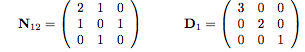
\includegraphics[scale=0.8]{disj2.png} 


\end{frame}
%%%%%%%%%%%%%%%%%%%%%%%%%%%%%%%%%%%

\begin{frame}{Tableau disjonctif joint}

 \begin{table}
\begin{tabular}{cc}

 & $\mathcal{X}(n \times m)= {X}_1\vert  {X}_2 \ldots  \vert{X}_p$ \\
& $m= m_1+\ldots +m_p$
 
\end{tabular} 
\end{table} 

\textbf{Exemple}
Pour les variables précédentes, on a le tableau disjonctif joint suivant

\centering 
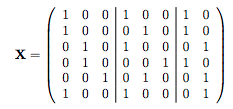
\includegraphics[scale=0.8]{disj3.png} 

Chaque somme de lignes vaut 3. Les sommes de colonnes
valent $$ (3 \ \ 2 \ \ 1 \lvert 3 \ \ 2 \ \ 1 \lvert 3 \ \ 3 )$$
\end{frame}

%%%%%%%%%%%%%%%%%%%%%%%%%%%%%%%%%%%

\begin{frame}{Le tableau de Burt}

 C'est un super-tableau de contingence des variables
$X_1, . . . , X_p$, formé de tableaux de contingence et de
matrices d'effectifs marginaux. : \\~\\

\centering
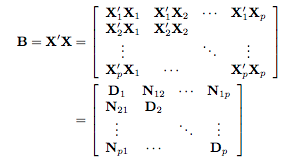
\includegraphics[scale=0.5]{Disj4} 
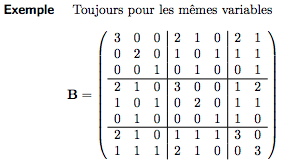
\includegraphics[scale=0.5]{Disj5} 

\end{frame}

%%%%%%%%%%%%%%%%%%%%%%%%%%%%%%%%%%%

\begin{frame}{L'ACM : une AFC sur tableau disjonctif}

Chercher une représentation des $m_1+\ldots+m_p$
catégories comme points d'un espace de faible dimension.\\ ~\\

\textbf{Méthode }  Faire une AFC sur le tableau disjonctif joint   
$$ \mathcal{X}(n \times m)= {X}_1\vert  {X}_2\vert  \ldots  \vert{X}_p $$

 

 

\end{frame}

%%%%%%%%%%%%%%%%%%%%%%%%%%%%%%%%%%%

\begin{frame}{L'ACM : une AFC sur tableau disjonctif}

 \begin{itemize}
 \item \textbf{Les lignes }:  La somme des éléments de chaque ligne de $\mathcal{X}$
est égale à p. Le \textbf{tableau des profils-lignes} est donc $\frac{1}{p} \mathcal{X}$\\~\\


\item \textbf{Les colonnes} : la somme des éléments de chaque colonne de $\mathcal{X}$ est égale à l'effectif marginal de la catégorie correspondante.\\~\\
 \end{itemize}

Le tableau des profils colonnes est donc $\mathcal{X}D^{-1}$
où $D$ est la matrice diagonale par blocs.

\centering

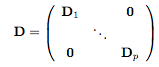
\includegraphics[scale=0.8]{Disj6} 

\end{frame}


%%%%%%%%%%%%%%%%%%%%%%%%%%%%%%%%%%%

\begin{frame}{Les coordonnées factorielles des catégories}
\centering 
 On note $a_k = (a_{1k}, \ldots , a_{pk})$ vecteur à $m_1 + \ldots + m_p$ composantes des coordonnées factorielles des catégories sur l'axe k. \\~\\
 
 \textbf{Calcul de l'AFC sur $\mathcal{X}$  }\\~\\
 
La matrice des profils lignes est $$\frac{1}{p} \mathcal{X}$$

et  celle des profils colonnes $$\mathcal{X}D^{-1}$$ . 

 
 
\end{frame}


%%%%%%%%%%%%%%%%%%%%%%%%%%%%%%%%%%%

\begin{frame}{Les coordonnées factorielles des catégories}
\centering 
 On note $a_k = (a_{1k}, \ldots , a_{pk})$ vecteur à $m_1 + \ldots + m_p$ \textcolor{blue}{composantes des coordonnées factorielles des catégories sur l'axe k}. \\~\\
 
% \textbf{Calcul de l'AFC sur $\mathcal{X}$  }\\
 
\textbf{$a_k$ est vecteur propre} de $$(\mathcal{X}D^{-1})' \frac{1}{p} \mathcal{X}=\frac{1}{p}{D^{-1}} \mathcal{X}' \mathcal{X}=  \frac{1}{p}{D^{-1}} B$$ 

l’équation des coordonnées des catégories est donc 
 $$\frac{1}{p}{D^{-1}} Ba_k=\mu_k a_k  $$ 
 Avec la convention de normalisation suivantes
  $$\frac{1}{np} {a_k}'Da_k=\mu_k   $$ 

 
 
\end{frame}


%%%%%%%%%%%%%%%%%%%%%%%%%%%%%%%%%%%

\begin{frame}{Resolution cas p=2}
 
\centering 

 On note $a = (a_{1},  a_{2})$ vecteur à $m_1 +  m_2$ composantes   factorielles des catégorie et $\mu_k$ la valeur propre correspondante. \\ \ \\
 

 
 \textbf{Calcul de l'AFC sur $\mathcal{X}$}\\ \ \\
 
 
  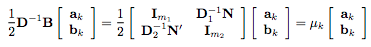
\includegraphics[scale=0.8]{AFC1} 
  
 
\end{frame}


%%%%%%%%%%%%%%%%%%%%%%%%%%%%%%%%%%%

\begin{frame}{Resolution cas p=2}
 
\centering 

 On note $a = (a_{1},  a_{2})$ vecteur à $m_1 +  m_2$ composantes   factorielles et $\mu_k$ la valeur propre correspondante.\\ \ \\
 
 
 % 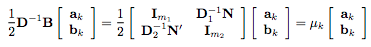
\includegraphics[scale=0.6]{AFC1} \\ \ \\
  
  On obtient les équations
  
   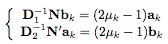
\includegraphics[scale=0.7]{AFC2} \\ \ \\
  
 et donc on retrouve les coordonnées des modalités de lignes
et de colonnes dans l'AFC classique (avec 
$\mu_k =(2\lambda_k - 1)^2) $

 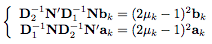
\includegraphics[scale=0.7]{AFC3} 
 
\end{frame}




%%%%%%%%%%%%%%%%%%%%%%%%%%%%%%%%%%%


\begin{frame}{Différences ACM/AFC pour p = 2}
 
\begin{itemize}
 \item \textbf{ Nombre de valeurs propres} : on a a priori $m_1 + m_2 - 2$ valeurs propres non nulles, En particulier pour chaque $\lambda_k$, on a deux $\mu_k$ possibles\\~\\
 
 \includegraphics[scale=0.6]{AFC4} 
 
 On ne garde donc que les valeurs $\mu_k >0.5$\\~\\
 
 \item \textbf{Inertie} : l'interprétation de la part d'inertie expliquée par
les valeurs propres est maintenant très différente. \\~\\
\textcolor{blue}{En particulier les valeurs propres qui étaient très séparées dans
l’AFC de N le sont beaucoup moins dans celle de X.}
 
 \end{itemize} 
 
\end{frame}

%%%%%%%%%%%%%%%%%%%%%%%%%%%%%%%%%%
\subsection{Aspects pratiques}

\begin{frame}{Formules barycentriques}
 
 \begin{itemize}
 \centering
 \item  Les coordonnées des individus 
 
  \includegraphics[scale=0.7]{AFC5} 
  
  Avec variance 
  
  \includegraphics[scale=0.7]{AFC6} 
 

 \item  Les coordonnées des catégories
 
 \includegraphics[scale=0.7]{AFC7} 
 
 \end{itemize}
 
 
\end{frame}


 

%%%%%%%%%%%%%%%%%%%%%%%%%%%%%%%%%%


%%%%%%%%%%%%%%%%%%%%%%%%%%%%%%%%%%


\begin{frame}{ Barycentres et représentation }
 
 \begin{itemize}
 
 \item  Les points représentatifs des catégories sont barycentres des groupes d'individus.
 
 \item Moyennes comme $c_k$ est une variable de moyenne nulle, la formule de barycentre indique que pour chaque variable $X_i$
les coordonnées de ses catégories  sont de moyenne nulle. 
 
 \item  Pour que les catégories se trouvent visuellement
au barycentre des individus qui les représentent on peut
remplacer $a_k$ 

\centering

 \includegraphics[scale=0.7]{AFC8} 
 
 \end{itemize}
 
 
\end{frame}

%%%%%%%%%%%%%%%%%%%%%%%%%%%%%%%%%%

\begin{frame}{ Sélection des axes }
 
 \begin{itemize}
 \item  règle courante : garder les axes tels que $\mu_k > \frac{1}{p}$ (la moyenne des valeurs propres est $\frac{1}{p}$).
 \item  les axes intéressants sont ceux que l'on peut interpréter,
en regardant les contributions des variables actives et les valeurs-tests associées aux variables supplémentaires.
 \item En pratique on se contente souvent d’interpréter le
premier plan principal.
 \end{itemize}
 
 
\end{frame}

%%%%%%%%%%%%%%%%%%%%%%%%%%%%%%%%%%


%%%%%%%%%%%%%%%%%%%%%%%%%%%%%%%%%%

\begin{frame}{ Sélection des axes }
 
 \begin{itemize}
 \item   Si $n_j$ est l’effectif de la catégorie $j$ et $a_{jk}$ sa coordonnée sur l’axe factoriel $k$, alors

\centering  
  
 \includegraphics[scale=0.7]{AFC9} 
 
 
 \item  \textbf{Catégorie} La contribution de la catégorie j à l’axe factoriel

est : 

\centering 

 \includegraphics[scale=0.7]{AFC10} 
 
 \item  \textbf{Variable :} la contribution totale de la variable $\xi_v$ à l'axe factoriel est 
 
  \includegraphics[scale=0.7]{AFC11} 
  
   
 \end{itemize}
 
 
\end{frame}



%%%%%%%%%%%%%%%%%%%%%%%%%%%%%%%%%%

\begin{frame}{ Contribution d’un individu }
 
 \begin{itemize}
 
 \centering  
 \item   Elle est égale pour l'individu i à 
 
 \includegraphics[scale=.8]{AFC12} 


\item Qualité de la représentation pour le sous-espace formé
par les  premier axes, la qualité de la représentation de
l'individu i est le cosinus carré habituel
   
    \includegraphics[scale=.8]{AFC13} 
 \end{itemize}
 
 
\end{frame}

%%%%%%%%%%%%%%%%%%%%%%%%%%%%%%%%%%
\subsection{Cas pratique}
\begin{frame}{Exemple}

 \includegraphics[scale=.5]{ACM1} 


\centering Projection des variables qualitatives sur le premier plan\\~\\

\textcolor{blue}{Que pensez vous de l'inertie porté par le premier plan ?}

\end{frame}

\begin{frame}{Exemple}

 \includegraphics[scale=.5]{ACM2} 
 
 \centering Inertie des différents\\~\\

\textcolor{blue}{Que pensez vous du nombre d'axes ?}

\end{frame}

\begin{frame}{Exemple}

 \includegraphics[scale=.5]{ACM3} 

\centering Projection des modalités des variables qualitatives \\~\\

\textcolor{blue}{Interprétez ?}

\end{frame}

\begin{frame}{Exemple : Utilisation des composantes factorielles}
\centering 
 \includegraphics[scale=.4]{ACM4} 

\centering CAH sur les composantes factorielles \\~\\

\textcolor{blue}{Interprétez ?}

\end{frame}

 
\end{document}